\documentclass[a4paper,journal]{IEEEtran}
\usepackage{tikz}
\usepackage{pgfplots}
\usepackage{xcolor}
\usepackage{color, colortbl}
\usepackage{amsmath}
\usepackage{amsfonts, amssymb}
\usepackage{amsmath}
\usepackage{algpseudocode,amsmath}
\pgfplotsset{compat=1.17}

\begin{document}

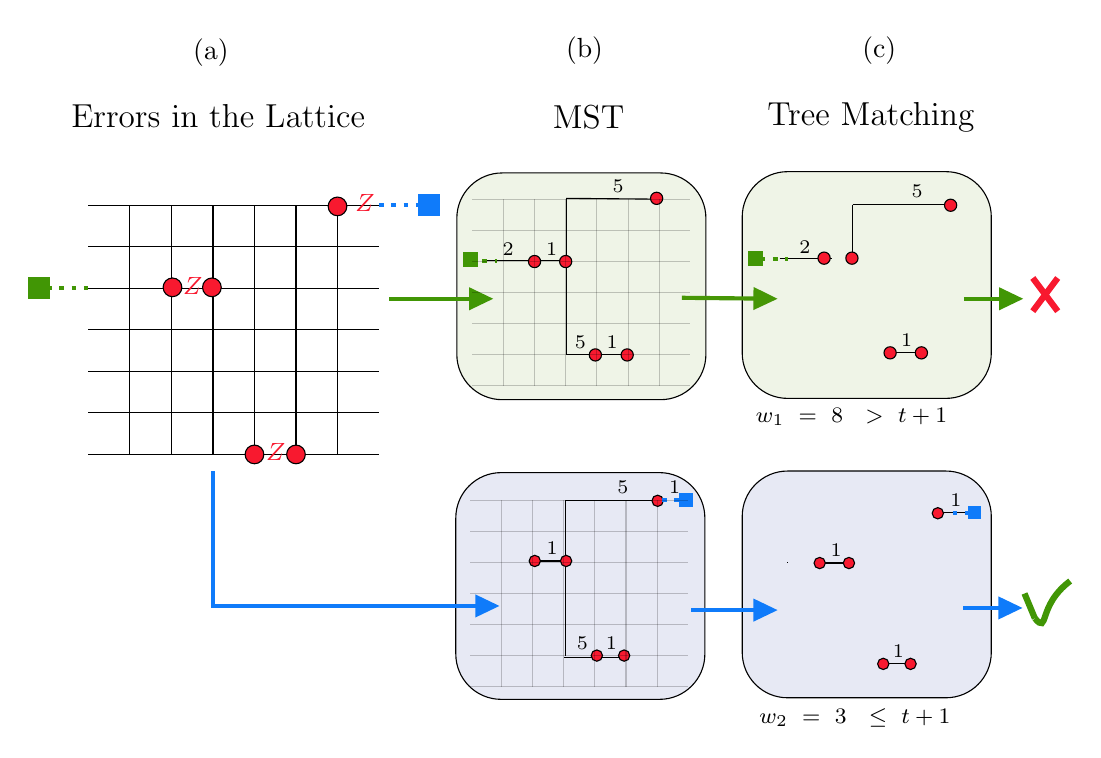
\begin{tikzpicture}[x=0.75pt,y=0.75pt,yscale=-1,xscale=1]

\draw  [fill={rgb, 255:red, 231; green, 233; blue, 244 }  ,fill opacity=1 ] (217,253.61) .. controls (217,241.54) and (226.78,231.76) .. (238.85,231.76) -- (315.15,231.76) .. controls (327.22,231.76) and (337,241.54) .. (337,253.61) -- (337,319.15) .. controls (337,331.22) and (327.22,341) .. (315.15,341) -- (238.85,341) .. controls (226.78,341) and (217,331.22) .. (217,319.15) -- cycle ;
\draw  [fill={rgb, 255:red, 231; green, 233; blue, 244 }  ,fill opacity=1 ] (355,252.85) .. controls (355,240.78) and (364.78,231) .. (376.85,231) -- (453.15,231) .. controls (465.22,231) and (475,240.78) .. (475,252.85) -- (475,318.39) .. controls (475,330.46) and (465.22,340.24) .. (453.15,340.24) -- (376.85,340.24) .. controls (364.78,340.24) and (355,330.46) .. (355,318.39) -- cycle ;
\draw  [fill={rgb, 255:red, 239; green, 244; blue, 231 }  ,fill opacity=1 ] (355,108.61) .. controls (355,96.54) and (364.78,86.76) .. (376.85,86.76) -- (453.15,86.76) .. controls (465.22,86.76) and (475,96.54) .. (475,108.61) -- (475,174.15) .. controls (475,186.22) and (465.22,196) .. (453.15,196) -- (376.85,196) .. controls (364.78,196) and (355,186.22) .. (355,174.15) -- cycle ;
\draw  [fill={rgb, 255:red, 239; green, 244; blue, 231 }  ,fill opacity=1 ] (217.5,109.23) .. controls (217.5,97.16) and (227.28,87.38) .. (239.35,87.38) -- (315.65,87.38) .. controls (327.72,87.38) and (337.5,97.16) .. (337.5,109.23) -- (337.5,174.77) .. controls (337.5,186.84) and (327.72,196.62) .. (315.65,196.62) -- (239.35,196.62) .. controls (227.28,196.62) and (217.5,186.84) .. (217.5,174.77) -- cycle ;
\draw    (40,103) -- (180,103) ;
\draw    (40,123) -- (180,123) ;
\draw    (40,143) -- (180,143) ;
\draw    (40,163) -- (180,163) ;
\draw    (40,183) -- (180,183) ;
\draw    (40,203) -- (180,203) ;
\draw    (40,223) -- (180,223) ;
\draw    (160,103) -- (160,223) ;
\draw    (140,103) -- (140,223) ;
\draw    (120,103) -- (120,223) ;
\draw    (100,103) -- (100,223) ;
\draw    (80,103) -- (80,223) ;
\draw    (60,103) -- (60,223) ;

\draw  [fill={rgb, 255:red, 248; green, 25; blue, 47 }  ,fill opacity=1 ] (155.5,103.5) .. controls (155.5,101.01) and (157.51,99) .. (160,99) .. controls (162.49,99) and (164.5,101.01) .. (164.5,103.5) .. controls (164.5,105.99) and (162.49,108) .. (160,108) .. controls (157.51,108) and (155.5,105.99) .. (155.5,103.5) -- cycle ;
\draw  [fill={rgb, 255:red, 248; green, 25; blue, 47 }  ,fill opacity=1 ] (76,142.5) .. controls (76,140.01) and (78.01,138) .. (80.5,138) .. controls (82.99,138) and (85,140.01) .. (85,142.5) .. controls (85,144.99) and (82.99,147) .. (80.5,147) .. controls (78.01,147) and (76,144.99) .. (76,142.5) -- cycle ;
\draw  [fill={rgb, 255:red, 248; green, 25; blue, 47 }  ,fill opacity=1 ] (95,142.5) .. controls (95,140.01) and (97.01,138) .. (99.5,138) .. controls (101.99,138) and (104,140.01) .. (104,142.5) .. controls (104,144.99) and (101.99,147) .. (99.5,147) .. controls (97.01,147) and (95,144.99) .. (95,142.5) -- cycle ;
\draw  [fill={rgb, 255:red, 248; green, 25; blue, 47 }  ,fill opacity=1 ] (115.5,223) .. controls (115.5,220.51) and (117.51,218.5) .. (120,218.5) .. controls (122.49,218.5) and (124.5,220.51) .. (124.5,223) .. controls (124.5,225.49) and (122.49,227.5) .. (120,227.5) .. controls (117.51,227.5) and (115.5,225.49) .. (115.5,223) -- cycle ;
\draw  [fill={rgb, 255:red, 248; green, 25; blue, 47 }  ,fill opacity=1 ] (135.5,223) .. controls (135.5,220.51) and (137.51,218.5) .. (140,218.5) .. controls (142.49,218.5) and (144.5,220.51) .. (144.5,223) .. controls (144.5,225.49) and (142.49,227.5) .. (140,227.5) .. controls (137.51,227.5) and (135.5,225.49) .. (135.5,223) -- cycle ;
\draw [color={rgb, 255:red, 15; green, 123; blue, 250 }  ,draw opacity=1 ][line width=1.5]  [dash pattern={on 1.69pt off 2.76pt}]  (180,103) -- (200,103) ;
\draw [color={rgb, 255:red, 65; green, 150; blue, 5 }  ,draw opacity=1 ][line width=1.5]  [dash pattern={on 1.69pt off 2.76pt}]  (20,143) -- (40,143) ;
\draw  [color={rgb, 255:red, 15; green, 123; blue, 250 }  ,draw opacity=1 ][fill={rgb, 255:red, 15; green, 123; blue, 250 }  ,fill opacity=1 ] (199,98) -- (209,98) -- (209,108) -- (199,108) -- cycle ;
\draw  [color={rgb, 255:red, 65; green, 150; blue, 5 }  ,draw opacity=1 ][fill={rgb, 255:red, 65; green, 150; blue, 5 }  ,fill opacity=1 ] (11,138) -- (21,138) -- (21,148) -- (11,148) -- cycle ;
\draw [color={rgb, 255:red, 65; green, 150; blue, 5 }  ,draw opacity=1 ][line width=1.5]    (185,148) -- (231,148) ;
\draw [shift={(235,148)}, rotate = 180] [fill={rgb, 255:red, 65; green, 150; blue, 5 }  ,fill opacity=1 ][line width=0.08]  [draw opacity=0] (11.61,-5.58) -- (0,0) -- (11.61,5.58) -- cycle    ;
\draw [color={rgb, 255:red, 15; green, 123; blue, 250 }  ,draw opacity=1 ][line width=1.5]    (100,231) -- (100,296) -- (234,296) ;
\draw [shift={(238,296)}, rotate = 180] [fill={rgb, 255:red, 15; green, 123; blue, 250 }  ,fill opacity=1 ][line width=0.08]  [draw opacity=0] (11.61,-5.58) -- (0,0) -- (11.61,5.58) -- cycle    ;
\draw    (270.18,99.61) -- (302.51,99.9) -- (314,100) ;
\draw    (229.96,129.76) -- (270.83,129.76) ;
\draw    (270.18,175.06) -- (296.63,175.06) ;
\draw    (270.18,99.61) -- (270.18,175.06) ;
\draw  [fill={rgb, 255:red, 248; green, 25; blue, 47 }  ,fill opacity=1 ] (310.82,99.61) .. controls (310.82,97.99) and (312.14,96.67) .. (313.77,96.67) .. controls (315.39,96.67) and (316.71,97.99) .. (316.71,99.61) .. controls (316.71,101.24) and (315.39,102.56) .. (313.77,102.56) .. controls (312.14,102.56) and (310.82,101.24) .. (310.82,99.61) -- cycle ;
\draw  [fill={rgb, 255:red, 248; green, 25; blue, 47 }  ,fill opacity=1 ] (252,130.06) .. controls (252,128.43) and (253.32,127.12) .. (254.94,127.12) .. controls (256.57,127.12) and (257.88,128.43) .. (257.88,130.06) .. controls (257.88,131.68) and (256.57,133) .. (254.94,133) .. controls (253.32,133) and (252,131.68) .. (252,130.06) -- cycle ;
\draw  [fill={rgb, 255:red, 248; green, 25; blue, 47 }  ,fill opacity=1 ] (267,130.06) .. controls (267,128.43) and (268.32,127.12) .. (269.94,127.12) .. controls (271.57,127.12) and (272.88,128.43) .. (272.88,130.06) .. controls (272.88,131.68) and (271.57,133) .. (269.94,133) .. controls (268.32,133) and (267,131.68) .. (267,130.06) -- cycle ;
\draw  [fill={rgb, 255:red, 248; green, 25; blue, 47 }  ,fill opacity=1 ] (281.31,175.06) .. controls (281.31,173.43) and (282.63,172.12) .. (284.25,172.12) .. controls (285.88,172.12) and (287.19,173.43) .. (287.19,175.06) .. controls (287.19,176.68) and (285.88,178) .. (284.25,178) .. controls (282.63,178) and (281.31,176.68) .. (281.31,175.06) -- cycle ;
\draw  [fill={rgb, 255:red, 248; green, 25; blue, 47 }  ,fill opacity=1 ] (296.63,175.06) .. controls (296.63,173.43) and (297.95,172.12) .. (299.58,172.12) .. controls (301.2,172.12) and (302.52,173.43) .. (302.52,175.06) .. controls (302.52,176.68) and (301.2,178) .. (299.58,178) .. controls (297.95,178) and (296.63,176.68) .. (296.63,175.06) -- cycle ;
\draw [color={rgb, 255:red, 65; green, 150; blue, 5 }  ,draw opacity=1 ][line width=1.5]  [dash pattern={on 1.69pt off 2.76pt}]  (223.88,129.76) -- (236.96,129.76) ;
\draw  [color={rgb, 255:red, 65; green, 150; blue, 5 }  ,draw opacity=1 ][fill={rgb, 255:red, 65; green, 150; blue, 5 }  ,fill opacity=1 ] (220.73,125.73) -- (227.27,125.73) -- (227.27,132.27) -- (220.73,132.27) -- cycle ;
\draw    (269.81,245.04) -- (316.39,245.04) ;
\draw    (255.05,274.33) -- (268.41,274.33) ;
\draw    (269.2,320.64) -- (296.71,320.64) ;
\draw    (269.81,245.04) -- (269.81,319.91) ;
\draw  [fill={rgb, 255:red, 248; green, 25; blue, 47 }  ,fill opacity=1 ] (311.51,245.34) .. controls (311.51,243.83) and (312.73,242.61) .. (314.24,242.61) .. controls (315.75,242.61) and (316.98,243.83) .. (316.98,245.34) .. controls (316.98,246.85) and (315.75,248.07) .. (314.24,248.07) .. controls (312.73,248.07) and (311.51,246.85) .. (311.51,245.34) -- cycle ;
\draw  [fill={rgb, 255:red, 248; green, 25; blue, 47 }  ,fill opacity=1 ] (252.32,274.33) .. controls (252.32,272.82) and (253.55,271.59) .. (255.05,271.59) .. controls (256.56,271.59) and (257.79,272.82) .. (257.79,274.33) .. controls (257.79,275.84) and (256.56,277.06) .. (255.05,277.06) .. controls (253.55,277.06) and (252.32,275.84) .. (252.32,274.33) -- cycle ;
\draw  [fill={rgb, 255:red, 248; green, 25; blue, 47 }  ,fill opacity=1 ] (267.41,274.33) .. controls (267.41,272.82) and (268.64,271.59) .. (270.15,271.59) .. controls (271.66,271.59) and (272.88,272.82) .. (272.88,274.33) .. controls (272.88,275.84) and (271.66,277.06) .. (270.15,277.06) .. controls (268.64,277.06) and (267.41,275.84) .. (267.41,274.33) -- cycle ;
\draw  [fill={rgb, 255:red, 248; green, 25; blue, 47 }  ,fill opacity=1 ] (282.22,319.91) .. controls (282.22,318.4) and (283.44,317.18) .. (284.95,317.18) .. controls (286.46,317.18) and (287.69,318.4) .. (287.69,319.91) .. controls (287.69,321.42) and (286.46,322.64) .. (284.95,322.64) .. controls (283.44,322.64) and (282.22,321.42) .. (282.22,319.91) -- cycle ;
\draw  [fill={rgb, 255:red, 248; green, 25; blue, 47 }  ,fill opacity=1 ] (295.37,319.91) .. controls (295.37,318.4) and (296.59,317.18) .. (298.1,317.18) .. controls (299.61,317.18) and (300.83,318.4) .. (300.83,319.91) .. controls (300.83,321.42) and (299.61,322.64) .. (298.1,322.64) .. controls (296.59,322.64) and (295.37,321.42) .. (295.37,319.91) -- cycle ;
\draw [color={rgb, 255:red, 15; green, 123; blue, 250 }  ,draw opacity=1 ][line width=1.5]  [dash pattern={on 1.69pt off 2.76pt}]  (316.39,245.04) -- (328.53,245.04) ;
\draw  [color={rgb, 255:red, 15; green, 123; blue, 250 }  ,draw opacity=1 ][fill={rgb, 255:red, 15; green, 123; blue, 250 }  ,fill opacity=1 ] (324.93,242) -- (331,242) -- (331,248.07) -- (324.93,248.07) -- cycle ;
\draw [color={rgb, 255:red, 15; green, 123; blue, 250 }  ,draw opacity=1 ][line width=1.5]    (330.47,298) -- (368,298) ;
\draw [shift={(372,298)}, rotate = 180] [fill={rgb, 255:red, 15; green, 123; blue, 250 }  ,fill opacity=1 ][line width=0.08]  [draw opacity=0] (11.61,-5.58) -- (0,0) -- (11.61,5.58) -- cycle    ;
\draw [color={rgb, 255:red, 70; green, 150; blue, 6 }  ,draw opacity=1 ][line width=1.5]    (325.95,147.53) -- (368,147.96) ;
\draw [shift={(372,148)}, rotate = 180.59] [fill={rgb, 255:red, 70; green, 150; blue, 6 }  ,fill opacity=1 ][line width=0.08]  [draw opacity=0] (11.61,-5.58) -- (0,0) -- (11.61,5.58) -- cycle    ;
\draw    (450.52,251.04) -- (462.39,251.04) ;
\draw    (393.05,275.33) -- (406.41,275.33) ;
\draw    (423.57,323.91) -- (435.31,323.91) ;
\draw    (376.81,274.9) -- (376.81,275.27) ;
\draw  [fill={rgb, 255:red, 248; green, 25; blue, 47 }  ,fill opacity=1 ] (446.51,251.34) .. controls (446.51,249.83) and (447.73,248.61) .. (449.24,248.61) .. controls (450.75,248.61) and (451.98,249.83) .. (451.98,251.34) .. controls (451.98,252.85) and (450.75,254.07) .. (449.24,254.07) .. controls (447.73,254.07) and (446.51,252.85) .. (446.51,251.34) -- cycle ;
\draw  [fill={rgb, 255:red, 248; green, 25; blue, 47 }  ,fill opacity=1 ] (389.59,275.33) .. controls (389.59,273.82) and (390.81,272.59) .. (392.32,272.59) .. controls (393.83,272.59) and (395.05,273.82) .. (395.05,275.33) .. controls (395.05,276.84) and (393.83,278.06) .. (392.32,278.06) .. controls (390.81,278.06) and (389.59,276.84) .. (389.59,275.33) -- cycle ;
\draw  [fill={rgb, 255:red, 248; green, 25; blue, 47 }  ,fill opacity=1 ] (403.68,275.33) .. controls (403.68,273.82) and (404.91,272.59) .. (406.41,272.59) .. controls (407.92,272.59) and (409.15,273.82) .. (409.15,275.33) .. controls (409.15,276.84) and (407.92,278.06) .. (406.41,278.06) .. controls (404.91,278.06) and (403.68,276.84) .. (403.68,275.33) -- cycle ;
\draw  [fill={rgb, 255:red, 248; green, 25; blue, 47 }  ,fill opacity=1 ] (420.22,323.91) .. controls (420.22,322.4) and (421.44,321.18) .. (422.95,321.18) .. controls (424.46,321.18) and (425.69,322.4) .. (425.69,323.91) .. controls (425.69,325.42) and (424.46,326.64) .. (422.95,326.64) .. controls (421.44,326.64) and (420.22,325.42) .. (420.22,323.91) -- cycle ;
\draw  [fill={rgb, 255:red, 248; green, 25; blue, 47 }  ,fill opacity=1 ] (433.37,323.91) .. controls (433.37,322.4) and (434.59,321.18) .. (436.1,321.18) .. controls (437.61,321.18) and (438.83,322.4) .. (438.83,323.91) .. controls (438.83,325.42) and (437.61,326.64) .. (436.1,326.64) .. controls (434.59,326.64) and (433.37,325.42) .. (433.37,323.91) -- cycle ;
\draw [color={rgb, 255:red, 15; green, 123; blue, 250 }  ,draw opacity=1 ][line width=1.5]  [dash pattern={on 1.69pt off 2.76pt}]  (456.39,251.04) -- (468.53,251.04) ;
\draw  [color={rgb, 255:red, 15; green, 123; blue, 250 }  ,draw opacity=1 ][fill={rgb, 255:red, 15; green, 123; blue, 250 }  ,fill opacity=1 ] (463.93,248) -- (470,248) -- (470,254.07) -- (463.93,254.07) -- cycle ;
\draw    (408.18,102.61) -- (456.71,102.61) ;
\draw    (372.96,128.76) -- (398.29,128.76) ;
\draw    (426.76,174.06) -- (440.64,174.06) ;
\draw    (408.18,102.61) -- (408.18,127.74) ;
\draw  [fill={rgb, 255:red, 248; green, 25; blue, 47 }  ,fill opacity=1 ] (452.46,102.94) .. controls (452.46,101.32) and (453.78,100) .. (455.4,100) .. controls (457.03,100) and (458.35,101.32) .. (458.35,102.94) .. controls (458.35,104.57) and (457.03,105.88) .. (455.4,105.88) .. controls (453.78,105.88) and (452.46,104.57) .. (452.46,102.94) -- cycle ;
\draw  [fill={rgb, 255:red, 248; green, 25; blue, 47 }  ,fill opacity=1 ] (391.49,128.44) .. controls (391.49,126.81) and (392.81,125.49) .. (394.44,125.49) .. controls (396.06,125.49) and (397.38,126.81) .. (397.38,128.44) .. controls (397.38,130.06) and (396.06,131.38) .. (394.44,131.38) .. controls (392.81,131.38) and (391.49,130.06) .. (391.49,128.44) -- cycle ;
\draw  [fill={rgb, 255:red, 248; green, 25; blue, 47 }  ,fill opacity=1 ] (404.91,128.44) .. controls (404.91,126.81) and (406.23,125.49) .. (407.86,125.49) .. controls (409.48,125.49) and (410.8,126.81) .. (410.8,128.44) .. controls (410.8,130.06) and (409.48,131.38) .. (407.86,131.38) .. controls (406.23,131.38) and (404.91,130.06) .. (404.91,128.44) -- cycle ;
\draw  [fill={rgb, 255:red, 248; green, 25; blue, 47 }  ,fill opacity=1 ] (423.31,174.06) .. controls (423.31,172.43) and (424.63,171.12) .. (426.26,171.12) .. controls (427.88,171.12) and (429.2,172.43) .. (429.2,174.06) .. controls (429.2,175.68) and (427.88,177) .. (426.26,177) .. controls (424.63,177) and (423.31,175.68) .. (423.31,174.06) -- cycle ;
\draw  [fill={rgb, 255:red, 248; green, 25; blue, 47 }  ,fill opacity=1 ] (438.39,174.06) .. controls (438.39,172.43) and (439.71,171.12) .. (441.33,171.12) .. controls (442.95,171.12) and (444.27,172.43) .. (444.27,174.06) .. controls (444.27,175.68) and (442.95,177) .. (441.33,177) .. controls (439.71,177) and (438.39,175.68) .. (438.39,174.06) -- cycle ;
\draw [color={rgb, 255:red, 65; green, 150; blue, 5 }  ,draw opacity=1 ][line width=1.5]  [dash pattern={on 1.69pt off 2.76pt}]  (363.89,128.76) -- (376.96,128.76) ;
\draw  [color={rgb, 255:red, 65; green, 150; blue, 5 }  ,draw opacity=1 ][fill={rgb, 255:red, 65; green, 150; blue, 5 }  ,fill opacity=1 ] (358,125.49) -- (364.54,125.49) -- (364.54,132.03) -- (358,132.03) -- cycle ;
\draw [color={rgb, 255:red, 15; green, 123; blue, 250 }  ,draw opacity=1 ][line width=1.5]    (461.47,296.96) -- (486,296.96) ;
\draw [shift={(490,296.96)}, rotate = 180] [fill={rgb, 255:red, 15; green, 123; blue, 250 }  ,fill opacity=1 ][line width=0.08]  [draw opacity=0] (11.61,-5.58) -- (0,0) -- (11.61,5.58) -- cycle    ;
\draw [color={rgb, 255:red, 65; green, 150; blue, 5 }  ,draw opacity=1 ][line width=1.5]    (461.81,148) -- (486.35,148) ;
\draw [shift={(490.35,148)}, rotate = 180] [fill={rgb, 255:red, 65; green, 150; blue, 5 }  ,fill opacity=1 ][line width=0.08]  [draw opacity=0] (11.61,-5.58) -- (0,0) -- (11.61,5.58) -- cycle    ;
\draw [color={rgb, 255:red, 248; green, 25; blue, 47 }  ,draw opacity=1 ][line width=2.25]    (495,138) -- (507,154) ;
\draw [color={rgb, 255:red, 248; green, 25; blue, 47 }  ,draw opacity=1 ][line width=2.25]    (507,138) -- (495,154) ;
\draw [color={rgb, 255:red, 65; green, 150; blue, 5 }  ,draw opacity=1 ][line width=2.25]    (491,290) -- (496,302) ;
\draw [color={rgb, 255:red, 65; green, 150; blue, 5 }  ,draw opacity=1 ][line width=2.25]    (496,302) .. controls (503,310) and (496.96,296) .. (513,284) ;
\draw [color={rgb, 255:red, 0; green, 0; blue, 0 }  ,draw opacity=0.21 ]   (225,100) -- (330,100) ;
\draw [color={rgb, 255:red, 0; green, 0; blue, 0 }  ,draw opacity=0.21 ]   (225,115) -- (330,115) ;
\draw [color={rgb, 255:red, 0; green, 0; blue, 0 }  ,draw opacity=0.21 ]   (225,130) -- (330,130) ;
\draw [color={rgb, 255:red, 0; green, 0; blue, 0 }  ,draw opacity=0.21 ]   (225,145) -- (330,145) ;
\draw [color={rgb, 255:red, 0; green, 0; blue, 0 }  ,draw opacity=0.21 ]   (225,160) -- (330,160) ;
\draw [color={rgb, 255:red, 0; green, 0; blue, 0 }  ,draw opacity=0.21 ]   (225,175) -- (330,175) ;
\draw [color={rgb, 255:red, 0; green, 0; blue, 0 }  ,draw opacity=0.21 ]   (225,190) -- (330,190) ;
\draw [color={rgb, 255:red, 0; green, 0; blue, 0 }  ,draw opacity=0.21 ]   (315,100) -- (315,190) ;
\draw [color={rgb, 255:red, 0; green, 0; blue, 0 }  ,draw opacity=0.21 ]   (300,100) -- (300,190) ;
\draw [color={rgb, 255:red, 0; green, 0; blue, 0 }  ,draw opacity=0.21 ]   (285,100) -- (285,190) ;
\draw [color={rgb, 255:red, 0; green, 0; blue, 0 }  ,draw opacity=0.21 ]   (270,100) -- (270,190) ;
\draw [color={rgb, 255:red, 0; green, 0; blue, 0 }  ,draw opacity=0.21 ]   (255,100) -- (255,190) ;
\draw [color={rgb, 255:red, 0; green, 0; blue, 0 }  ,draw opacity=0.21 ]   (240,100) -- (240,190) ;


\draw [color={rgb, 255:red, 0; green, 0; blue, 0 }  ,draw opacity=0.21 ]   (224,245) -- (329,245) ;
\draw [color={rgb, 255:red, 0; green, 0; blue, 0 }  ,draw opacity=0.21 ]   (224,260) -- (329,260) ;
\draw [color={rgb, 255:red, 0; green, 0; blue, 0 }  ,draw opacity=0.21 ]   (224,275) -- (329,275) ;
\draw [color={rgb, 255:red, 0; green, 0; blue, 0 }  ,draw opacity=0.21 ]   (224,290) -- (329,290) ;
\draw [color={rgb, 255:red, 0; green, 0; blue, 0 }  ,draw opacity=0.21 ]   (224,305) -- (329,305) ;
\draw [color={rgb, 255:red, 0; green, 0; blue, 0 }  ,draw opacity=0.21 ]   (224,320) -- (329,320) ;
\draw [color={rgb, 255:red, 0; green, 0; blue, 0 }  ,draw opacity=0.21 ]   (224,335) -- (329,335) ;
\draw [color={rgb, 255:red, 0; green, 0; blue, 0 }  ,draw opacity=0.21 ]   (314,245) -- (314,335) ;
\draw [color={rgb, 255:red, 0; green, 0; blue, 0 }  ,draw opacity=0.21 ]   (299,245) -- (299,335) ;
\draw [color={rgb, 255:red, 0; green, 0; blue, 0 }  ,draw opacity=0.21 ]   (284,245) -- (284,335) ;
\draw [color={rgb, 255:red, 0; green, 0; blue, 0 }  ,draw opacity=0.21 ]   (269,245) -- (269,335) ;
\draw [color={rgb, 255:red, 0; green, 0; blue, 0 }  ,draw opacity=0.21 ]   (254,245) -- (254,335) ;
\draw [color={rgb, 255:red, 0; green, 0; blue, 0 }  ,draw opacity=0.21 ]   (239,245) -- (239,335) ;



% Text Node
\draw (362,344.36) node [anchor=north west][inner sep=0.75pt]  [font=\footnotesize]  {$w_2 \ =\ 3\ \ \leq \ t + 1$};
% Text Node
\draw (360.35,199.4) node [anchor=north west][inner sep=0.75pt]  [font=\footnotesize]  {$w_1 \ =\ 8\ \  >\ t + 1$};
% Text Node
\draw (102.5,60) node  [font=\normalsize] [align=left] {{\large Errors in the Lattice}};
% Text Node
\draw (281,60.5) node  [font=\normalsize] [align=left] {{\large MST}};
% Text Node
\draw (417,60.5) node   [align=left] {{\large Tree Matching}};
% Text Node
\draw (99,29.5) node   [align=left] {(a)};
% Text Node
\draw (279,28.5) node   [align=left] {(b)};
% Text Node
\draw (421,28.5) node   [align=left] {(c)};
% Text Node
\draw (242.22,124) node  [font=\scriptsize]  {$2$};
% Text Node
\draw (263.22,124) node  [font=\scriptsize]  {$1$};
% Text Node
\draw (295.22,94) node  [font=\scriptsize]  {$5$};
% Text Node
\draw (292.33,169.12) node  [font=\scriptsize]  {$1$};
% Text Node
\draw (277,169) node  [font=\scriptsize]  {$5$};
% Text Node
\draw (385.22,123) node  [font=\scriptsize]  {$2$};
% Text Node
\draw (439.22,96) node  [font=\scriptsize]  {$5$};
% Text Node
\draw (434.22,168) node  [font=\scriptsize]  {$1$};
% Text Node
\draw (322.45,239) node  [font=\scriptsize]  {$1$};
% Text Node
\draw (297.45,239) node  [font=\scriptsize]  {$5$};
% Text Node
\draw (263.45,268) node  [font=\scriptsize]  {$1$};
% Text Node
\draw (292,314) node  [font=\scriptsize]  {$1$};
% Text Node
\draw (278,314) node  [font=\scriptsize]  {$5$};
% Text Node
\draw (400.22,269) node  [font=\scriptsize]  {$1$};
% Text Node
\draw (430.22,318) node  [font=\scriptsize]  {$1$};
% Text Node
\draw (458,245) node  [font=\scriptsize]  {$1$};
% Text Node
\draw (173.22,102) node  [font=\small,color={rgb, 255:red, 248; green, 25; blue, 47 }  ,opacity=1 ]  {$Z$};
% Text Node
\draw (90.22,142) node  [font=\small,color={rgb, 255:red, 248; green, 25; blue, 47 }  ,opacity=1 ]  {$Z$};
% Text Node
\draw (130.22,222) node  [font=\small,color={rgb, 255:red, 248; green, 25; blue, 47 }  ,opacity=1 ]  {$Z$};


\end{tikzpicture}

\end{document}